\chapter{Introducción}

En la actualidad, la seguridad de la información se ha convertido en un pilar
fundamental para el correcto funcionamiento de la sociedad digital. El aumento
constante en el volumen de datos transmitidos a través de redes de comunicación,
la expansión de los dispositivos conectados y la necesidad de proteger tanto la
privacidad como la integridad de la información han impulsado el desarrollo de
técnicas criptográficas cada vez más sofisticadas. Dentro de este amplio campo,
los \textit{cifrados de flujo} ocupan un lugar destacado debido a su eficiencia,
su sencillez conceptual y a su capacidad para adaptarse a escenarios en los que
la velocidad y el bajo consumo de recursos resultan esenciales.

\section*{Contexto y motivación}

El cifrado de flujo se caracteriza por combinar el texto plano con una secuencia
pseudoaleatoria de bits, denominada \textit{keystream}, generalmente mediante la
operación XOR. A diferencia de los cifrados en bloque, que procesan la
información en bloques de longitud fija, los cifrados de flujo trabajan de forma
bit a bit, lo que permite en muchos casos un procesamiento más rápido y una
implementación más ligera en dispositivos con recursos limitados.

\begin{figure}[h]
\centering
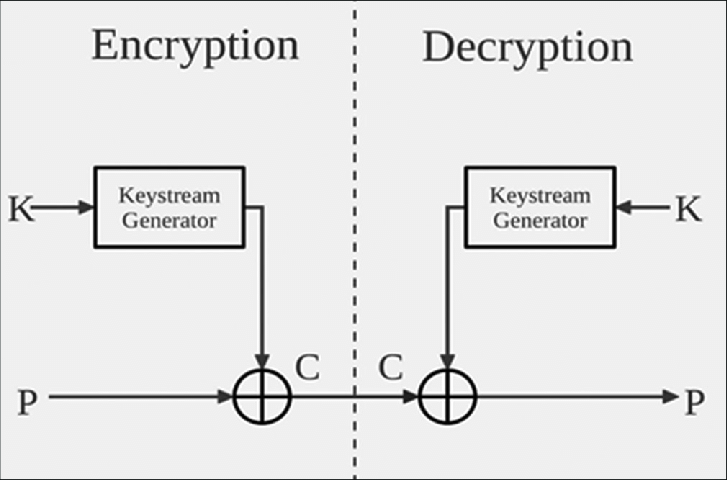
\includegraphics[width=0.8\textwidth]{figures/stream_cipher_scheme.png}
\caption{Esquema simplificado de un cifrador de flujo: el texto plano se combina
con un flujo de claves generado por un LFSR o un combinador de LFSR mediante XOR.}
\end{figure}


Por estas razones, los cifrados de flujo han sido ampliamente utilizados en aplicaciones
de comunicaciones móviles, protocolos de transmisión en tiempo real y sistemas
embebidos.

\begin{table}[h]
\centering
\begin{tabular}{l|c|c}
\textbf{Característica} & \textbf{Cifrado en bloque} & \textbf{Cifrado de flujo} \\
\hline
Unidad de operación & Bloques de $n$ bits & Bits individuales \\
Flexibilidad & Menor & Mayor \\
Velocidad en hardware & Alta & Muy alta \\
Ejemplos & AES, DES, Blowfish & RC4, A5/1, Salsa20 \\
\end{tabular}
\caption{Comparación entre cifrado en bloque y cifrado de flujo.}
\end{table}


No obstante, el gran reto que plantean estos cifrados radica en la construcción
del generador de flujo de claves. Si la secuencia generada presenta patrones,
redundancias o estructuras predecibles, un atacante puede explotar dichas
regularidades para recuperar el mensaje original o incluso reconstruir el
estado interno del generador. En consecuencia, el diseño de generadores de
secuencias pseudoaleatorias con buenas propiedades estadísticas y elevada
complejidad constituye un área de investigación activa dentro de la
criptografía aplicada.

Además, este trabajo se enmarca como una ampliación de estudios previos,
incorporando un conjunto más amplio de pruebas estadísticas y comparativas. La
motivación principal es evaluar de forma más exhaustiva las secuencias generadas
por LFSR y combinadores, con el fin de obtener una visión más completa de sus
fortalezas y limitaciones. Con ello se busca no solo validar resultados
anteriores, sino también aportar nuevos elementos de análisis que permitan
profundizar en la calidad y seguridad de estos generadores.

\subsection*{Antecedentes históricos}

El estudio de los cifradores de flujo y de los registros de desplazamiento de
retroalimentación lineal (LFSR) tiene sus raíces en los primeros trabajos de
Claude Shannon en la década de 1940, cuando se establecieron los fundamentos
teóricos de la criptografía moderna. Shannon introdujo la noción de
\textit{confusión} y \textit{difusión} como propiedades esenciales para la
seguridad de un sistema de cifrado, lo que influyó en el diseño posterior de
primitivas tanto de bloque como de flujo.

Durante los años 1950 y 1960, los LFSR comenzaron a utilizarse en sistemas de
comunicaciones y en generación de códigos de corrección de errores, gracias a su
simplicidad de implementación y a la posibilidad de producir secuencias de largo
período conocidas como \textit{m-secuencias}. Su bajo coste en hardware los
convirtió en una opción atractiva para dispositivos de telecomunicaciones y
aplicaciones militares.

En la década de 1980, los cifradores de flujo experimentaron un auge con el
desarrollo de algoritmos como RC4, ampliamente adoptado en protocolos como WEP y
posteriormente en SSL/TLS. Aunque con el tiempo se descubrieron debilidades
críticas en su diseño, RC4 marcó un hito en la historia de la criptografía de
flujo por su simplicidad y eficiencia.

Paralelamente, los sistemas de telefonía móvil GSM introdujeron el algoritmo
A5/1, basado en múltiples LFSR combinados mediante funciones no lineales. Este
caso mostró tanto las ventajas como las limitaciones de los LFSR: aunque
permitieron implementar cifrado ligero en dispositivos con recursos muy
reducidos, investigaciones posteriores demostraron vulnerabilidades que podían
explotarse mediante ataques de correlación y criptoanálisis algebraico.

En la actualidad, aunque muchos sistemas modernos han migrado hacia cifradores
de bloque en modos de operación que emulan flujos (como AES en CTR), los
cifradores de flujo y los LFSR siguen siendo relevantes en entornos de recursos
restringidos, comunicaciones en tiempo real y aplicaciones embebidas. Además,
siguen constituyendo un área de investigación activa como base para la
construcción de generadores pseudoaleatorios eficientes y seguros.


\subsection*{Limitaciones prácticas y retos actuales}

El diseño de un cifrador de flujo plantea retos que van más allá del rendimiento.
En la práctica, un generador debe satisfacer simultáneamente requisitos de
\emph{robustez} (resistencia frente a ataques), \emph{portabilidad} (facilidad de
integración en plataformas heterogéneas) y \emph{mantenibilidad} (claridad del
modelo y facilidad de verificación). En sistemas embebidos e IoT, además, la
seguridad compite con presupuestos estrictos de energía y memoria, lo que obliga
a optar por construcciones ligeras sin sacrificar propiedades estadísticas.

Desde el punto de vista criptográfico, la dificultad reside en garantizar que el
flujo de claves sea indistinguible de un proceso aleatorio ideal para cualquier
adversario computacionalmente acotado. Esto excluye, por ejemplo, generadores
puramente lineales: aunque produzcan secuencias de gran periodo y buena
dispersión, su estructura algebraica facilita ataques que reconstruyen el estado
interno a partir de un número finito de observaciones.

\subsection*{Aplicaciones y escenarios de uso}

Los cifradores de flujo destacan en:
\begin{itemize}
    \item \textbf{Comunicaciones en tiempo real}: voz y vídeo donde la latencia
    es crítica y la granularidad bit a bit evita rellenos y modos de operación
    complejos.
    \item \textbf{Sistemas embebidos e IoT}: sensores alimentados por batería y
    microcontroladores de baja potencia que requieren primitivas ligeras.
    \item \textbf{Enlaces inalámbricos y satelitales}: donde la sencillez del
    hardware y la alta tasa de bits favorecen generadores simples y eficientes.
\end{itemize}

En todos estos casos, el desafío consiste en equilibrar eficiencia y seguridad,
minimizando tanto los sesgos estadísticos como la predictibilidad estructural.


\section*{Pseudoaleatoriedad en criptografía}

La noción de \textit{aleatoriedad} es fundamental en criptografía. Una
secuencia verdaderamente aleatoria debería ser impredecible y carecer de todo
patrón discernible. Sin embargo, la generación de aleatoriedad perfecta suele
depender de fenómenos físicos (como ruido térmico, radiactividad o fluctuaciones
cuánticas) que no siempre están disponibles ni son fáciles de integrar en
sistemas digitales.

Por ello, se recurre habitualmente a la \textit{pseudoaleatoriedad}, es decir, a
secuencias generadas por algoritmos deterministas a partir de un estado inicial
o semilla, que presentan la apariencia de ser aleatorias. Aunque en esencia son
predecibles si se conoce el algoritmo y la semilla, un buen generador debe
producir secuencias indistinguibles de la aleatoriedad verdadera para un
observador sin esa información.

En este contexto, resultan especialmente relevantes los \textbf{postulados de
Golomb}, que establecen tres propiedades básicas que deberían cumplir las
secuencias pseudoaleatorias: (1) un número equilibrado de ceros y unos, (2) una
distribución adecuada de rachas de bits consecutivos y (3) una autocorrelación
desplazada lo más cercana posible a cero. Estas condiciones permiten evaluar
rápidamente si una secuencia se asemeja a un comportamiento aleatorio ideal.

Además de los postulados de Golomb, en la práctica se emplean baterías de
pruebas estadísticas desarrolladas por la NIST (Instituto Nacional de Estándares y Tecnologías),
que incluyen tests de frecuencia, longitud de rachas, correlación, complejidad lineal,
entre otros. Estas pruebas resultan fundamentales para determinar si un generador
es apto para su uso en criptografía.

\subsection*{Criterios de indistinguibilidad y pruebas estadísticas}

El objetivo práctico de la pseudoaleatoriedad es la \emph{indistinguibilidad}:
que ningún algoritmo eficiente pueda diferenciar una secuencia generada de otra
verdaderamente aleatoria con ventaja significativa. En la práctica, esta noción
se aproxima mediante pruebas estadísticas que evalúan propiedades parciales (no
exhaustivas) del flujo.

Entre las pruebas más utilizadas se encuentran las de la batería NIST SP~800--22.
A continuación se detallan aquellas relevantes para este trabajo, junto con una
breve interpretación operativa de sus estadísticos y p--valores:

\paragraph{Frecuencia (monobit).}
Sea $x_i \in \{0,1\}$ y $\tilde{x}_i = 2x_i-1 \in \{-1,1\}$. El estadístico
es $S_n = \sum_{i=1}^n \tilde{x}_i$ y el p--valor se aproxima por
$p=\operatorname{erfc}\!\big(|S_n|/\sqrt{2n}\big)$. Valores pequeños indican sesgo
global hacia 0 o 1.

\paragraph{Frecuencia por bloques.}
Dividiendo la secuencia en bloques de tamaño $M$, se calcula, para cada bloque
$j$, la fracción $\pi_j$ de unos. El contraste $\chi^2$ sobre $\{\pi_j\}$ detecta
sesgos \emph{locales}. Un generador puede pasar monobit y fallar aquí si alterna
zonas sesgadas.

\paragraph{Rachas (runs).}
Define $V_n = 1 + \sum_{i=1}^{n-1} \mathbf{1}_{\{x_i \neq x_{i+1}\}}$. Este test
compara $V_n$ con su esperanza bajo balance. Detecta exceso o defecto de
transiciones, revelando agregación o alternancia artificial.

\paragraph{Sumas acumulativas (CUSUM).}
Considera la caminata $S_k=\sum_{i=1}^k \tilde{x}_i$ y su desviación máxima
$M_n=\max_{1\le k\le n}|S_k|$. Un $M_n$ grande sugiere un sesgo \emph{acumulado}
no visible en un prefijo corto.

\paragraph{Entropía aproximada (ApEn).}
Compara la distribución de patrones de longitud $m$ y $m{+}1$ a través de sus
entropías empíricas; p--valores bajos indican regularidades de corto alcance.

\paragraph{Universal de Maurer.}
Mide la \emph{compresibilidad} esperada de la secuencia. Patrones repetidos o
estructura redundante reducen el p--valor.

\paragraph{Serial.}
Evalúa la frecuencia de todas las palabras de longitud $m$ (y a menudo $m{+}1$).
Detecta asimetrías o vacíos en el espectro de patrones cortos.

\medskip
En todos los casos, se adopta un umbral $\alpha=0.01$: si $p\ge \alpha$ se
\emph{acepta} la hipótesis de aleatoriedad para esa prueba. Fallar de forma
consistente un subconjunto de tests sugiere la presencia de estructura
aprovechable por un atacante.


\section*{Registros LFSR}

Uno de los mecanismos más estudiados y empleados para la generación de
secuencias pseudoaleatorias es el \textit{Linear Feedback Shift Register}
(LFSR). Estos registros desplazan su estado interno en cada iteración y
calculan el nuevo bit de entrada como una combinación lineal (módulo 2) de
ciertos bits de la propia secuencia, definidos por un polinomio generador. Los
LFSR son extremadamente eficientes en hardware y software, lo que los convierte
en candidatos idóneos para sistemas de alta velocidad y entornos con recursos
limitados.

Históricamente, los LFSR han sido empleados en criptografía aplicada, en
sistemas de comunicaciones inalámbricas como GSM, en generación de códigos de
control de errores y en simulaciones de procesos estocásticos. Su atractivo
radica en su bajo coste computacional, pero su estructura lineal conlleva
también importantes debilidades: dado un número suficiente de bits de salida, es
posible reconstruir el polinomio de retroalimentación y el estado inicial
mediante algoritmos como Berlekamp-Massey. Además, un único LFSR suele fallar
en varios tests de aleatoriedad, lo que limita su uso directo en cifrado de
flujo.

\subsection*{Modelo algebraico y propiedades básicas}

Un LFSR binario de grado $m$ viene determinado por su vector de estado
$s^{(t)}=(s_0^{(t)},\dots,s_{m-1}^{(t)})\in\{0,1\}^m$ y por un conjunto de
\emph{taps} $T\subseteq \{0,\dots,m-1\}$. La actualización es lineal sobre
$\mathbb{F}_2$:
\[
s_0^{(t+1)} \;=\; \bigoplus_{i\in T} s_i^{(t)},\qquad
s_j^{(t+1)} \;=\; s_{j-1}^{(t)}\ \ (1\le j\le m-1),
\]
donde $\oplus$ denota la suma módulo 2. Esta dinámica equivale al polinomio de
retroalimentación $f(x)=1+\sum_{i\in T} x^{i} + x^m$. Si $f(x)$ es \emph{primitivo}
sobre $\mathbb{F}_2$, el LFSR genera una \emph{m-secuencia} de periodo máximo
$2^m{-}1$ (para cualquier estado inicial no nulo).

Las m-secuencias satisfacen los postulados de Golomb en el límite y presentan
un espectro binario plano, pero su \emph{complejidad lineal} es exactamente $m$:
existe un LFSR de longitud $m$ (el propio) que reproduce la secuencia. Esto
implica que, observando un prefijo suficientemente largo, es posible reconstruir
el estado y el polinomio mediante procedimientos como Berlekamp--Massey.

\subsection*{Complejidad lineal y recuperación de estado}

La complejidad lineal $L$ de una secuencia binaria es la longitud del LFSR más
corto capaz de generarla. El algoritmo de Berlekamp--Massey estima $L$ a partir
de un prefijo $x_1,\dots,x_n$ en tiempo $O(n^2)$, devolviendo además un
polinomio de conexión candidato. En términos criptográficos, $L$ acota el
esfuerzo necesario para reconstruir el generador por medios puramente lineales;
valores bajos de $L$ hacen a la secuencia predecible con pocos bits observados.

Estas limitaciones motivan el uso de \emph{combinadores no lineales} de varios
LFSR, buscando aumentar $L$ y romper correlaciones explotables, sin abandonar la
eficiencia estructural de los registros.


\section*{Estado del arte y generadores combinados}

Con el fin de superar estas limitaciones, la literatura ha propuesto múltiples
estrategias basadas en la combinación de varios LFSR mediante funciones no
lineales. Estos esquemas incrementan la complejidad del sistema y dificultan los
intentos de predicción del flujo generado. Entre los ejemplos más representativos
se encuentran:

\begin{itemize}
    \item El \textbf{generador Shrinking}, que utiliza un LFSR de control para
          decidir qué bits de otro LFSR se incluyen en la secuencia final.
    \item El \textbf{generador de Geffe}, que combina tres LFSR mediante una
          función booleana no lineal que incrementa la complejidad de la
          secuencia producida.
    \item El \textbf{generador de Mayoría}, en el que la salida depende del
          valor mayoritario de varios LFSR en cada instante.
\end{itemize}

Estos generadores, aunque aumentan la resistencia frente a ciertos ataques,
requieren un análisis detallado mediante métricas estadísticas y estructurales
para determinar si la mejora es realmente significativa respecto al uso de un
LFSR individual.

\subsection*{Ataques clásicos a generadores basados en LFSR}

La linealidad facilita varios vectores de ataque:
\begin{itemize}
    \item \textbf{Ataques de correlación}: cuando la salida combinada conserva
    correlación estadística con la salida de algún LFSR interno, es posible
    “desacoplar” el sistema probando estados parciales y maximizando verosimilitudes.
    \item \textbf{Ataques algebraicos}: expresando la salida como polinomios
    booleanos del estado, se plantean sistemas de ecuaciones sobre $\mathbb{F}_2$
    que, bajo ciertas condiciones, admiten resolución más rápida que la búsqueda
    exhaustiva.
    \item \textbf{Time–memory tradeoff}: técnicas que precalculan grandes tablas
    (por ejemplo, cadenas de estados) para acelerar la recuperación del estado
    durante un ataque en línea.
\end{itemize}

Estos ataques justifican dos líneas de defensa complementarias: (i) aumentar la
\emph{complejidad lineal} efectiva de la salida y (ii) reducir correlaciones
explotables entre la salida y los estados internos, tanto en promedio como en
subconjuntos de bits.


\section*{Objetivos del trabajo}

El objetivo general de este Trabajo Fin de Grado es \textbf{estudiar y optimizar
secuencias de bits pseudoaleatorias basadas en LFSR para su aplicación en
cifrado de flujo}. Para alcanzar este propósito se plantean los siguientes
objetivos específicos:

\begin{enumerate}
    \item Implementar en Python generadores basados en LFSR y sus variantes
        combinadas (Shrinking, Geffe y Mayorías).
    \item Generar secuencias de prueba de longitud suficiente para un análisis
        estadístico riguroso.
    \item Evaluar la calidad pseudoaleatoria de dichas secuencias mediante un
        conjunto de tests seleccionados de la batería por la NIST (Instituto
        Nacional de Estándares y Tecnologías), así como los postulados de Golomb.
    \item Calcular la complejidad lineal de las secuencias generadas empleando
        el algoritmo de Berlekamp-Massey.
    \item Comparar los resultados obtenidos entre diferentes configuraciones de
        LFSR y combinadores, analizando ventajas y limitaciones de cada caso.
    \item Ampliar el conjunto de pruebas estadísticas respecto a trabajos anteriores,
        incluyendo no solo los tests clásicos de la batería por la NIST (Instituto
        Nacional de Estándares y Tecnologías), sino también métricas adicionales
        que permitan una caracterización más precisa de las secuencias.
    \item Analizar críticamente las diferencias obtenidas respecto a estudios previos,
        valorando en qué medida los nuevos resultados confirman, refuerzan o
        contradicen conclusiones anteriores.

\end{enumerate}

\section*{Hipótesis y alcance}

La hipótesis de partida es que los LFSR individuales, aunque eficientes en
términos de implementación, presentan limitaciones tanto en complejidad lineal
como en propiedades pseudoaleatorias, lo que los hace vulnerables a ataques de
predicción o reconstrucción. No obstante, al combinar varios registros mediante
funciones no lineales, se espera obtener secuencias con mayor calidad
estadística y una complejidad superior, incrementando así la resistencia frente
a ataques criptoanalíticos.

El alcance de este trabajo se centra en el análisis de generadores en un entorno
software, sin abordar implementaciones hardware ni optimizaciones específicas
para plataformas embebidas. El estudio se focaliza en tres combinadores
representativos de la literatura —Shrinking, Geffe y Mayorías— y en un conjunto
de pruebas estadísticas seleccionadas que permitan valorar de forma fiable la
aleatoriedad y la complejidad de las secuencias producidas. A diferencia de
estudios previos, este trabajo no se limita a replicar experimentos, sino que
los amplía incorporando un mayor número de pruebas comparativas y métricas
adicionales, con el objetivo de ofrecer una caracterización más completa del
comportamiento de los generadores basados en LFSR. De este modo, el presente TFG
se plantea como una continuación y mejora de investigaciones anteriores en la
materia.

\section*{Terminología y notación}

\begin{table}[h]
\centering
\begin{tabular}{ll}
\toprule
Símbolo & Descripción \\
\midrule
$\mathbb{F}_2$ & Campo binario $\{0,1\}$ con suma XOR. \\
$x_1,\dots,x_n$ & Secuencia binaria de longitud $n$. \\
$\tilde{x}_i$ & Transformación $2x_i-1\in\{-1,1\}$. \\
$L$ & Complejidad lineal de una secuencia. \\
$f(x)$ & Polinomio de realimentación del LFSR. \\
$T$ & Conjunto de taps del LFSR. \\
$S_n$ & Estadístico monobit $\sum_{i=1}^n \tilde{x}_i$. \\
$M$ & Tamaño de bloque en frecuencia por bloques. \\
$\alpha$ & Nivel de significación (aquí $\alpha=0{.}01$). \\
$p$ & p--valor de una prueba estadística. \\
\bottomrule
\end{tabular}
\caption{Glosario mínimo de símbolos y términos utilizados.}
\end{table}

\section*{Metodología y reproducibilidad}

El estudio sigue una metodología empírico–comparativa con implementación en Python y control de semillas. El proceso se organiza en: (i) definición formal de generadores (LFSR y combinados), (ii) generación de secuencias con longitudes prefijadas, (iii) evaluación estadística (subset NIST) y estimación de complejidad lineal, y (iv) síntesis de resultados mediante medias, desviaciones estándar y tasas de aceptación para $\alpha=0{.}01$.

Se garantiza reproducibilidad mediante control de semillas, registro de parámetros de ejecución, separación de código/datos/resultados, exportación de tablas en CSV/\LaTeX{} y documentación de dependencias.

\section*{Criterios de evaluación y significación}

La comparación entre configuraciones se basa en:
\begin{itemize}
  \item Tasas de aceptación por prueba (umbral $\alpha=0{.}01$) agrupadas sobre múltiples semillas.
  \item Estadísticos agregados (media y desviación estándar) de p--valores por prueba y configuración.
  \item Complejidad lineal estimada por Berlekamp–Massey como indicador operativo de predictibilidad.
  \item Longitud efectiva de salida en combinadores con descarte (p.\,ej., Shrinking).
\end{itemize}
Se considera que una configuración mejora a otra cuando incrementa las tasas de aceptación sin sacrificar complejidad lineal ni longitud efectiva de forma significativa.

\section*{Casos de uso y escenarios de aplicación}

Se consideran tres dominios representativos:
\begin{itemize}
  \item Sensórica IoT con restricciones de energía y memoria.
  \item Streaming en tiempo real de voz/vídeo con baja latencia.
  \item Enlaces inalámbricos de alto caudal con hardware sencillo.
\end{itemize}
En estos contextos, combinadores basados en LFSR ofrecen un compromiso entre coste computacional y calidad estadística siempre que superen pruebas básicas y presenten alta complejidad lineal.

\section*{Limitaciones y amenazas a la validez}

\begin{itemize}
  \item Selección parcial de pruebas NIST; algunas debilidades podrían no detectarse.
  \item Dependencia del tamaño muestral y del número de repeticiones.
  \item Resultados condicionados a polinomios, semillas y longitudes escogidas.
  \item Ausencia de criptoanálisis activo más allá de medidas estadísticas y de complejidad lineal.
\end{itemize}
Estas amenazas se mitigan mediante multi–semilla, reporte de dispersión y documentación de parámetros para facilitar replicación.

\section*{Objetivos extendidos y aportaciones medibles}

\begin{itemize}
  \item Cobertura: ejecutar $r\geq 30$ repeticiones por configuración y semillas variadas.
  \item Longitudes: evaluar $n\in\{10^5,5\cdot 10^5,10^6\}$ para estudiar estabilidad de p--valores.
  \item Complejidad lineal: reportar la distribución empírica de $L$ por configuración.
  \item Reproducibilidad: publicar parámetros, semillas y resultados tabulados desde las ejecuciones.
\end{itemize}

\section*{Resumen del capítulo}

Se ha establecido el contexto y la motivación del uso de LFSR y combinadores en cifrado de flujo, junto con objetivos, alcance, metodología y criterios de evaluación. El Capítulo~2 desarrolla la pseudoaleatoriedad y las métricas empleadas; el Capítulo~3 aborda LFSR, complejidad lineal y generadores combinados; el Capítulo~4 presenta el experimento y los resultados; el Capítulo~5 ofrece conclusiones y líneas futuras.
